\documentclass[tikz,border=4pt]{standalone}
% Shared setup for the foundation-model diagrams, in the AFRICAST palette
\usepackage{fontspec}
\usepackage[sfdefault]{FiraSans}
\usepackage{amsmath}
\usepackage{unicode-math}
\setmathfont{Fira Math}
\usetikzlibrary{arrows.meta}
\definecolor{ink}{HTML}{1F2A36}
\definecolor{MonashBlue}{HTML}{3B75AC}
\definecolor{Orange}{HTML}{B5570F}
\color{ink}
\tikzset{every picture/.style={draw=ink,>=stealth}}
\hyphenpenalty=10000
\exhyphenpenalty=10000

\begin{document}
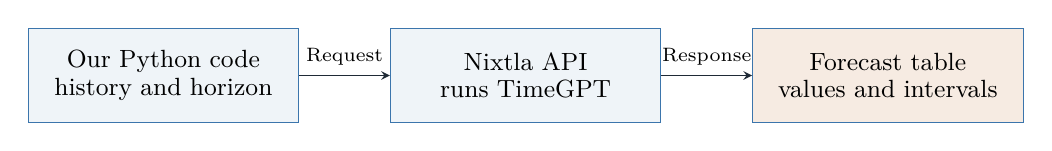
\begin{tikzpicture}[>=stealth,every node/.style={font=\fontsize{9}{10}\selectfont,align=center},
box/.style={draw=MonashBlue,fill=MonashBlue!8,text width=3.2cm,minimum height=1.2cm}]
\node[box] (a) at (0,0) {Our Python code\\history and horizon};
\node[box] (b) at (4.6,0) {Nixtla API\\runs TimeGPT};
\node[box,fill=Orange!12] (c) at (9.2,0) {Forecast table\\values and intervals};
\draw[->] (a)--node[above,font=\fontsize{7}{8}\selectfont]{Request}(b);\draw[->] (b)--node[above,font=\fontsize{7}{8}\selectfont]{Response}(c);
\end{tikzpicture}
\end{document}
